\section{最坏情形复杂度}
\label{sec:simplex-worst-case}

单纯形法有限终止，但有限不等于快。换基次数在最坏情况下能有多大，它和一次换基的代价是什么关系，实际表现又该怎样理解？

\paragraph{换基次数与每轮代价}
总运算量是两个因子的乘积：换基次数乘以每轮代价。第~\ref{sec:simplex-revised}节处理的是后者，稠密实现下每轮是$m$和$n$的低次多项式。本节讨论前者。基的个数最多是从$n$个下标中选$m$个的组合数，随规模指数增长，所以有限终止本身给不出多项式界。问题在于，算法会不会真的走那么多步。

\paragraph{Klee--Minty构造}
下面这族例子表明确实可能。第$n$个问题有$n$个变量和$n$个约束：
\begin{equation}
 \begin{aligned}
 \max\quad & z_n=\sum_{j=1}^n2^{n-j}x_j\\
 \text{s.t.}\quad & x_i+\sum_{j<i}2^{i-j+1}x_j\leq5^i,\quad i=1,\ldots,n,\\
 & \bm{x}\geq\bm{0}.
 \end{aligned}
 \label{eq:simplex-klee-minty}
\end{equation}
它属于Klee和Minty提出的压扁立方体构造\scite{math-klee1972simplex}。$n=2$时约束是$x_1\leq5$，$4x_1+x_2\leq25$，目标是$2x_1+x_2$。从原点出发，Dantzig规则选系数大的$x_1$，走到$(5,0)$；接着$x_2$入基，走到$(5,5)$；最后第一个松弛变量入基，走到$(0,25)$。四个顶点全被访问，如图~\ref{fig:simplex-klee-minty-plane}所示。

\begin{BookInlineFigure}
 \centering
 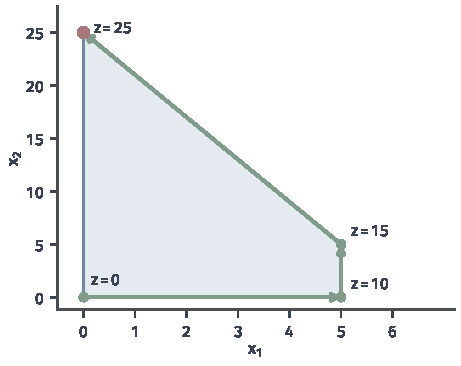
\includegraphics[width=78mm]{figures/05-optimization/01-linear-programming/matplotlib/simplex-klee-minty-plane/figure.pdf}
 \caption{$n=2$的Klee--Minty问题。可行域（浅蓝）有四个顶点，绿色路径依次访问全部四个，每个顶点旁标出目标值$z$，红点是最优解$(0,25)$。注意最优点其实与起点相邻，算法却绕了远路。}
 \label{fig:simplex-klee-minty-plane}
\end{BookInlineFigure}

$n=3$时情况相同，图~\ref{fig:simplex-klee-minty-cube}是可行域的示意。路径走完底面的四个顶点，上升一次，再把顶面的四个顶点反向走一遍。

\begin{BookInlineFigure}
 \centering
 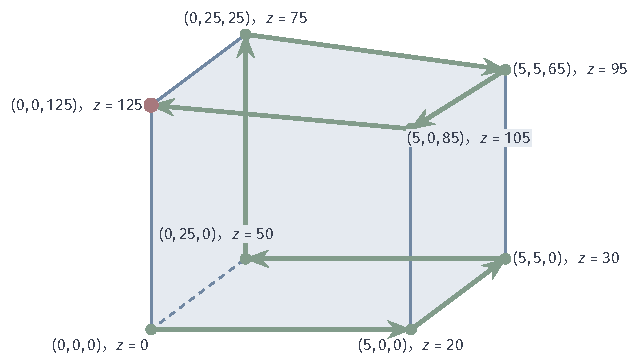
\includegraphics[width=108mm]{figures/05-optimization/01-linear-programming/tikz/simplex-klee-minty-cube/figure.pdf}
 \caption{$n=3$的Klee--Minty问题的示意，画成立方体，顶点坐标和目标值$z$是真实数据，比例不真实。绿色路径是Dantzig规则访问的顺序，共$7$次换基、走遍$8$个顶点，红点是最优解。}
 \label{fig:simplex-klee-minty-cube}
\end{BookInlineFigure}

这种“走完一面、再反着走一遍”的结构可以写成对$n$的归纳。为了写证明，先观察目标和约束之间的递推关系。记第$i$个松弛变量为$w_i$。由式~\eqref{eq:simplex-klee-minty}，第$n$个目标和第$n$个约束都可以用$z_{n-1}$表示：
\begin{equation}
 z_n=2z_{n-1}+x_n,\qquad w_n=5^n-x_n-4z_{n-1}.
 \label{eq:simplex-klee-minty-recursion}
\end{equation}
前$n-1$个约束恰好是第$n-1$个问题的约束，其中不含$x_n$和$w_n$。

下面用“字典”的语言：字典是把基变量和目标写成非基变量函数的表达式，也就是式~\eqref{eq:simplex-basic-form}和式~\eqref{eq:simplex-objective-form}的另一种叫法。最大化时，Dantzig规则选目标表达式中系数最大的正系数变量入基，这与最小化标准型中选最负的$s_j$是同一条规则。

\begin{theorem}[Klee--Minty问题的换基次数]
 \label{thm:simplex-klee-minty}
 对问题~\eqref{eq:simplex-klee-minty}，从全部松弛变量组成的基出发，Dantzig规则恰好经过$2^n-1$次换基到达最优解，最优值为$5^n$。
\end{theorem}

\begin{proof}
 对$n$归纳证明一个更强的命题。把从全松弛基出发、最大化$z_n$的运行称为上行，记为$U_n$；把从$U_n$的终点出发、最大化$-z_n$的运行称为下行，记为$D_n$。命题是：$U_n$和$D_n$各有$2^n-1$次换基；$U_n$过程中$z_n$从$0$增加到$5^n$，$D_n$过程中$z_n$从$5^n$减少到$0$并回到全松弛基；所有字典的目标系数都是整数。

 $n=1$时$z_1=x_1$，$w_1=5-x_1$。上行时$x_1$入基，一次换基后$z_1=5-w_1$。下行时目标是$-z_1=-5+w_1$，$w_1$入基，一次换基后$-z_1=-x_1$。命题成立。

 设命题对$n-1$成立，先看$U_n$。由式~\eqref{eq:simplex-klee-minty-recursion}，它分三段。

 第一段。设第$n-1$个问题的字典中$z_{n-1}$的系数为$d_k$，它们是整数。此时$z_n$的系数是$2d_k$，而$x_n$的系数是$1$。只要有$d_k>0$，就有$2d_k\geq2>1$，Dantzig规则的选择与$U_{n-1}$完全相同。第$n$行也不起限制作用，因为$x_n=0$且$z_{n-1}\leq5^{n-1}$，由式~\eqref{eq:simplex-klee-minty-recursion}得
 \[
  w_n\geq5^n-4\cdot5^{n-1}=5^{n-1}>0.
 \]
 所以算法照搬$U_{n-1}$，$2^{n-1}-1$次换基后$z_{n-1}=5^{n-1}$，所有$d_k\leq0$。

 第二段。此时只有$x_n$的系数为正，它入基。$x_n$只出现在第$n$行，所以$w_n$出基，$x_n=5^{n-1}$。这是一次换基。把$x_n=5^n-w_n-4z_{n-1}$代入$z_n$，目标变为
 \[
  z_n=5^n-w_n-2z_{n-1}.
 \]

 第三段。现在$w_n$的系数是$-1$，其余系数是$-2d_k$，后者正是$D_{n-1}$的目标$-z_{n-1}$放大$2$倍，$w_n$的系数为负，不会入基。第$n$行现在是$x_n=5^n-w_n-4z_{n-1}$，$w_n=0$时$x_n\geq5^{n-1}>0$，不起限制作用。所以算法照搬$D_{n-1}$，$2^{n-1}-1$次换基后$z_{n-1}=0$，所有系数非正，算法停止，此时$z_n=5^n$。

 三段合计$2(2^{n-1}-1)+1=2^n-1$次换基。

 再看$D_n$，它从$-z_n=-5^n+w_n+2z_{n-1}$开始，$z_{n-1}$的字典是全松弛基。第一段中$w_n$的系数是$1$，其余是$2d_k$，同样的比较说明算法照搬$U_{n-1}$，第$n$行$x_n\geq5^{n-1}>0$不起限制作用。第二段只有$w_n$的系数为正，它入基，$x_n$出基，代入后目标变为
 \[
  -z_n=-x_n-2z_{n-1}.
 \]
 第三段照搬$D_{n-1}$，第$n$行$w_n\geq5^{n-1}>0$不起限制作用，最后回到全松弛基，$z_n=0$。

 整数性由式~\eqref{eq:simplex-klee-minty-recursion}的递推保持，因为各段目标都是归纳假设中的整数系数乘$\pm2$再加上系数为$\pm1$的$x_n$或$w_n$。归纳完成。
\end{proof}

证明的要点在于系数的差距：前$n-1$个变量的系数翻倍，所以只要还有事可做，Dantzig规则就不会理会$x_n$；右端$5^i$的快速增长保证第$n$行不起限制作用。换一种规则结论就可能改变，图~\ref{fig:simplex-klee-minty-counts}(a)中Bland规则在这族例子上的步数少一些，但这只说明这族例子不是专门针对Bland规则构造的，其他构造同样能使Bland规则走指数多步。是否存在一条换基规则能保证多项式次换基，至今没有答案。

\begin{BookInlineFigure}
 \centering
 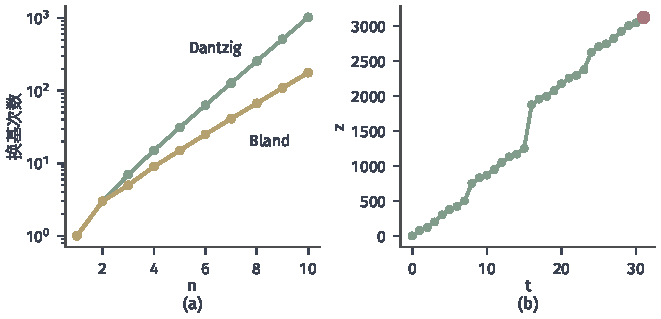
\includegraphics[width=112mm]{figures/05-optimization/01-linear-programming/matplotlib/simplex-klee-minty-counts/figure.pdf}
 \caption{Klee--Minty问题的实测结果，精确有理数运算。(a)~换基次数随$n$变化，纵轴取对数；绿线是Dantzig规则，恰为$2^n-1$；黄线是Bland规则。(b)~$n=5$时Dantzig规则各步的目标值，共$31$步，红点是最优值$3125$。}
 \label{fig:simplex-klee-minty-counts}
\end{BookInlineFigure}

\paragraph{最坏情形与实际表现}
定理~\ref{thm:simplex-klee-minty}是对一族特殊问题的结论，并不刻画算法在一般问题上的行为。长期的实践表明，单纯形法在大多数实际问题上的换基次数远小于组合数，常是约束数的不大的倍数。

图~\ref{fig:simplex-random-pivots}是一个小实验：$\bm{A},\bm{c}$的元素在$(0,1)$上独立均匀抽取，$\bm{b}=\bm{1}$，$m=n$，每种规模取$30$个随机种子。平均换基次数随规模温和增长，$m=320$时约$655$次，比Klee--Minty问题的指数增长慢得多。

\begin{BookInlineFigure}
 \centering
 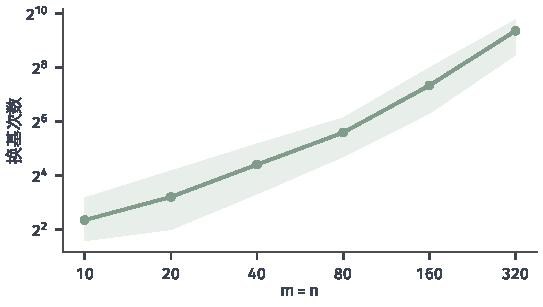
\includegraphics[width=92mm]{figures/05-optimization/01-linear-programming/matplotlib/simplex-random-pivots/figure.pdf}
 \caption{一种随机模型上Dantzig规则的换基次数，两轴都是对数刻度。绿线是$30$个随机种子的平均值，浅绿色带是最小值到最大值的范围。实验条件：$m=n$，$\bm{A},\bm{c}$的元素在$(0,1)$上独立均匀，$\bm{b}=\bm{1}$，起始基是全松弛基。}
 \label{fig:simplex-random-pivots}
\end{BookInlineFigure}

这个实验只说明这一随机模型上的情况，不能外推成对任意问题的保证。实际问题带有特定的结构，有时比随机模型容易，有时因退化严重而困难得多。理论上也有在特定随机扰动模型下给出多项式期望步数的结果，那些结论依赖扰动模型，并不告诉我们某一个具体实例要走多少步。

所以这里的两个判断要分开说：最坏情形下，Dantzig规则的换基次数可以随维数指数增长，这是定理；实际问题上换基次数通常不大，这是经验观察，没有无条件的平均复杂度保证。这个差别也是下一章研究多项式时间方法的原因之一。
